% Beamer template
% Author: Ozgur Taylan TURAN
% Delft University of Technology

\documentclass[aspectratio=169]{beamer}
\usepackage{/home/taylanot/texmf/tex/beamerthemetot}
% PACKAGES
\usepackage[english]{babel}
\usepackage{graphicx}
\usepackage{animate}
%\usepackage{calc}
\usepackage{calligra}
\usepackage[absolute,overlay]{textpos}
\usepackage[T1]{fontenc}
%\usefonttheme{serif}
\usefonttheme{professionalfonts}
\usepackage{amsmath}
\usepackage{palatino}
\usepackage{mathpazo}
\usepackage{graphicx}
%\usepackage{subfig}
\usepackage{tikz}
\usetikzlibrary{shapes,arrows}
\usepackage{xcolor}
\usepackage[T1]{fontenc}
%\usefonttheme{serif}
%\usepackage{titling}
\usepackage{graphicx}
%\usepackage{subfig}
%\usepackage{tikz}
%\usetikzlibrary{shapes,arrows}
\usepackage{mathtools}
\usepackage{cancel}
    
% BIB SETTINGS
\usepackage[backend=bibtex,firstinits=true,maxnames=30,maxcitenames=20,url=false,style=authoryear]{biblatex}
\bibliography{../../../archive_bib/library.bib}

\setlength\bibitemsep{0.3cm} % space between entries in the reference list
\renewcommand{\bibfont}{\normalfont\scriptsize}
\renewcommand{\cite}[1]{\footnote<.->[frame]{\fullcite{#1}}}
\setbeamertemplate{bibliography item}{}

\setbeamertemplate{navigation symbols}{} % remove navigation symbols

\usepackage{perpage} \MakePerPage{footnote}

 % COVER PAGE INFO   
\newcommand{\mytitle}{\color{White}\huge{\textbf{Coffee Talk \#4}}}
\newcommand{\mysubtitle}{\color{Pink}\Large{\textbf{Learning Rate Annealing Can Provably Help Generalization Even For Convex Problems}}}
\newcommand{\myauthor}{\color{White}\textcalligra{\LARGE Ozgur Taylan Turan}}
\newcommand{\authorlabel}{\small O.T. Turan}
\author{\authorlabel}


\begin{document}
% COVER PAGE
{
{
\def\beamer@entrycode{\vspace*{-\headheight}}
\setbeamertemplate{frametitle}[default][center]
\setbeamertemplate{navigation symbols}{}
\usebackgroundtemplate{
\includegraphics[width=\paperwidth,height=\paperheight]{cover/coverart.pdf}}

\begin{frame}[plain] 

\begin{minipage}{\textwidth}
	\centering{\mytitle} \\
	%\vspace{1cm}
	%\centering{\mysubtitle} \\
	\vspace{1cm}
	\centering{\color{White}November 15, 2021} \\
	\vspace{1cm}
	\centering{\myauthor}\\
\end{minipage}
\end{frame}
}

\setbeamercovered{transparent}
\setbeamertemplate{footline}{\usebeamertemplate*{minimal footline}}
\setbeamertemplate{headline}{\usebeamertemplate*{minimal headline}}
\def\beamer@entrycode{\vspace*{-\headheight}}
}
% MAIN
\setbeamercovered{transparent}


\begin{frame}
	\centering
	\mysubtitle\cite{Nakkiran2020b}
\end{frame}

\begin{frame}{Why This Paper?}
	\centering
	\begin{minipage}{0.8\textwidth}
			\centering
			 Simple, but not obvious observations...
	\end{minipage}
\end{frame}

\begin{frame}{Aim}
  \centering
	\begin{minipage}{0.7\textwidth}
		\centering
     Show that large initial learning rate can act as a regularizer! 
     \begin{itemize}
       \item Non-convex setting \cite{Li2019}
       \item Convex setting \cite{Nakkiran2020b}
      \end{itemize}
	\end{minipage}
\end{frame}

\begin{frame}{Non-Convex Setting \cite{Li2019}-\only<1>{A}\only<2>{B}\only<3>{C}\only<4>{D}\only<5>{E}}
  \centering
   \only<2>
  {
    \color{Pink}Claim 1: \color{Black} Small learning rate $\to$ easy-to-generalize and hard-to-fit patterns

    \color{Pink}Claim 2: \color{Black} Large learning rate $\to$ hard-to-generalize and easy-to-fit patterns

    \vspace{3cm}
    \color{Black} Complex theoretical and a small empirical investigation.
  }
  \includegraphics<1>[width=0.95\textwidth]{Figures/li_1}
  \includegraphics<3>[width=0.7\textwidth]{Figures/li_patch}

  \only<3> {CIFAR-10: 20\% No-patch, 16\% Only-patch, 60\% Image-with-patch }
  \includegraphics<4>[width=0.95\textwidth]{Figures/li_2}

  \only<4> {Small Gaussian-noise addition before activation layer have a regularizing effect on the small learning rate!}

  \only<5>
  {
    \color{Pink}Claim 3: \color{Black}Convex problems have unique minimum, so this effect cannot be observed!
  }
\end{frame}

\begin{frame}{Convex Setting \cite{Nakkiran2020b}}
  \only<1>
  {
  \begin{block}{\color{White}Problem}
    \begin{itemize}
      \item Assume a distribution $\mathcal{D}$ over $(x,y) \in \mathbb{R}^2x\mathbb{R}$
      \item Given $x\in\{\textbf{e}_1, \textbf{e}_2\}$ uniformly at random; $y = \langle\beta^*,x\rangle$ for ground truth $\mathbb{R}^2$
      \item Learn a linear model $\hat{y}:=\langle\beta,x\rangle$, where $\beta=(\beta_1,\beta_2)$
      \item Noting, population loss $\to$ $L_\mathcal{D}:= \mathbb{E}_D\Big[(\langle\beta,x\rangle-y)^2\Big]$
      \item And, empirical loss $\to$ $\hat{L}_n:= \frac{1}{n}\sum_{i}(\langle\beta,x_i\rangle-y_i)^2$ for drawn n samples from the distribution $\mathcal{D}$ 
    \end{itemize}
  \end{block}
  }
  \only<2-3>
  {
    \centering 
    \color{Pink} Assume you have $n=3$ with $(x_i,y_i)_{i=1}^3\to\{(\textbf{e}_1, \beta_1^*),(\textbf{e}_1, \beta_1^*),(\textbf{e}_2, \beta_2^*)\}$
    \only<2-3>
    {
    \begin{minipage}{0.45\textwidth}
        \begin{block}{\color{White}Empirical Loss}
          \centering
          $\hat{L}_n:=\frac{2}{3}(\beta_1-\beta_1^*)^2+\frac{1}{3}(\beta_2-\beta_2^*)^2$
        \end{block} 
    \end{minipage}%
  }
    \hspace{1cm}
    \only<3>
    {
    \begin{minipage}{0.5\textwidth}
      \begin{block}{\color{White}Population Loss}
          \centering
          $L_\mathcal{D}:=\frac{1}{2}(\beta_1-\beta_1^*)^2+\frac{1}{2}(\beta_2-\beta_2^*)^2$
        \end{block} 
    \end{minipage}
    }
  }
\end{frame}

\begin{frame}{Convex Setting \cite{Nakkiran2020b}}
\centering 
  \color{Pink} Start from 0-initialization and update with SGD until $\hat{L}_n=\varepsilon$ with small learning rate (a) and large learning rate with annealing (b)
  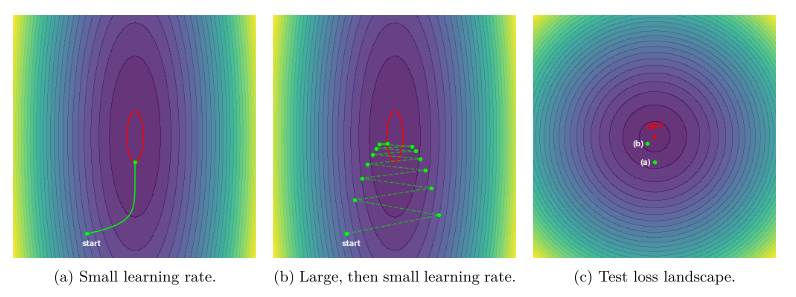
\includegraphics[width=0.7\textwidth]{Figures/exp}

  \only<2> {\color{Black} So, large learning rate is regularizing the high curvature update and allow better generalization performance.}
\end{frame}

\begin{frame}{Conclusions}
\begin{itemize}
  \item Learning rate can have a regularizing effect in both convex and non-convex settings, although reasons are different.
  \item Investigation of learning rate remains an open question in more complex settings.
\end{itemize}
\end{frame}

\end{document}

